%File: formatting-instruction.tex
\documentclass[letterpaper]{article}
% AAAI format packages
\usepackage{aaai}
\usepackage{times}
\usepackage{helvet}
\usepackage{courier}
% Additional packages
\usepackage{amsmath}
\usepackage{amssymb}
\usepackage{amsthm}
\usepackage{algorithm}
\usepackage{algorithmic}
\usepackage{graphicx}
\usepackage{comment}
\newtheorem{defn}{Definition}
\newtheorem{lemma}{Lemma}
\newtheorem{thm}{Theorem}
\newtheorem{cor}{Corollary}
\newtheorem{rul}{Expansion Rule}
% END Additional packages
\frenchspacing
\setlength{\pdfpagewidth}{8.5in}
\setlength{\pdfpageheight}{11in}
\pdfinfo{
/Title (Constraints on Frontier Expansion for Approximate Shortest Paths)
%/Author (Aram Ebtekar, Mike Phillips, Sven Koenig, Maxim Likhachev)
/Keywords (weighted A* search, parallel algorithm, heuristic)
}
\setcounter{secnumdepth}{0}  
 \begin{document}
% The file aaai.sty is the style file for AAAI Press 
% proceedings, working notes, and technical reports.
%
\title{Constraints on Frontier Expansion for Approximate Shortest Paths}
\author{Aram Ebtekar$^\dagger$ \and Mike Phillips$^\dagger$ \and Sven Koenig\thanks{University of Southern California, Los Angeles, CA 90089} \and Maxim Likhachev% <-this % stops a space
\thanks{Carnegie Mellon University, Pittsburgh, PA 15217}% <-this % stops a space
%
}
\author{ICAPS 2015 Submission 166}% anonymizer
\maketitle
\begin{abstract}
\begin{quote}
Given a consistent heuristic, the weighted A* search algorithm chooses an ordering of frontier expansions in such a way that an approximately optimal solution is found without needing any re-expansions.
wPA*SE is a recent parallel variant of A* which offers the same guarantee and can achieve a nearly linear speedup in the number of processor cores, provided expansions are sufficiently time-consuming to dominate the search runtime.
Much of the overhead of wPA*SE is due to careful selection of states to expand, as required to meet the theoretical guarantees.
In this work, we look at several criteria which sufficiently constrain the frontier's expansion.
In particular, we present novel extensions to wPA*SE that maintain speedups at faster expansion rates than wPA*SE allows.
They generalize the state expansion criterion so that more states are eligible for concurrent expansion, while also making the criterion cheaper to compute.
On the theoretical side, we prove the same guarantees on completeness and solution quality as wA* and wPA*SE, as well as a parallel time complexity result.
Experimentally, we obtain comparable performance to wPA*SE when expansions are very slow, and better performance as expansions become faster and the number of cores increases.
\end{quote}
\end{abstract}

\section{Introduction}

Breadth-first and depth-first search are generalized by a class of frontier-based search algorithms, differing mainly in the order by which states are selected from the frontier for expansion. In the weighted A* (wA*) algorithm, the choice combines a greedy goal-directed bias to reduce search time, with a breadth-first bias which ensures suboptimality bounded by a specified factor. When provided with a consistent heuristic, wA* takes care to expand a state only after finding an approximately optimal path reaching it. Thus, wA* can guarantee approximate optimality without ever re-expanding a state.

With the advent of multi-core processors, making use of parallelism has become a priority for algorithm designers. Parallel A* for Slow Expansions (PA*SE) \cite{phillips2014pa}, and its weighted generalization wPA*SE, offer nearly linear speedup in the number of cores, provided the search time is dominated by time-consuming expansions. Among parallel algorithms for graph search, wPA*SE stands out for meeting the same theoretical guarantee as wA*: approximate optimality without repeated expansions.

In this paper, we analyze in greater depth the conditions under which A* variants can meet this theoretical guarantee. This analysis naturally leads to Enhanced PA*SE (ePA*SE). Its performance at least rivals wPA*SE in general, and surpasses it when expansions times are faster or a lot of processor cores are available. This enables several theoretical results, which we also present. Our final result  shows how ePA*SE generalizes a parallel approximation algorithm for single-source shortest paths \cite{klein1997randomized}, providing time complexity bounds in the massively parallel limit.

DELETE: Finally, we present  Parallel Anytime Repairing A* (PARA*), a simultaneous improvement over both Anytime Repairing A* (ARA*) and ePA*SE. ARA* and PARA* are anytime search algorithms, gradually reducing the goal-directed bias to improve solution cost as much as planning time allows.

\section{Related Work}

Some early parallel versions of Dijkstra’s algorithm \cite{quinn86} and A* \cite{irani86} \cite{leifker85} worked by simultaneously expanding some number of states in the frontier with the lowest $g$ or $f$ values. These methods do not bound suboptimality on the first expansion, so they must allow re-expansions.
The approach of \cite{vidal10} performs well by increasing the number of threads if the goal is not found within some number of expansions, but they offer no guaranteed bounds on solution suboptimality.

There are several methods which split the frontier into multiple pieces for parallel processing.
Parallel Retracting A* (PRA*) \cite{evett95} uses a hash function to map each state to a processor.
Parallel Structured Duplicate Detection (PSDD) \cite{zhou07}
uses a state abstraction function to group states into
``nblocks".
Each processor takes an entire nblock and can expand all its states without locking, provided
that neighboring nblocks are not undergoing expansion.
Parallel Best-NBlock-First (PBNF) \cite{burns_10} fuses the two latter
approaches, running PRA* with a hashing function
based on PSDD state abstraction.
This avoids much of the thread locking in PRA*.
This approach has also been extended to weighted (bounded
sub-optimal) and anytime search.
A more recent algorithm based on PRA* hashing is Hash Distributed A* (HDA*) \cite{kishimoto09},
which uses asynchronous message passing to deliver hashed states between processors without blocking the sending thread.

Instead of parallelizing a single search algorithm, \cite{valenzano10} run a variety of planning algorithms in parallel.
By taking the quickest result, their solution quality is bounded by the worst quality bound among their set of search algorithms. Since the planners run independently of one another, the same state may be expanded multiple times.
Likewise, the preceding approaches must allow states to be re-expanded, perhaps exponentially many times, in order to guarantee bounded suboptimality. Weighted Parallel A* for Slow Expansions (wPA*SE) \cite{phillips2014pa}
is a recent approach which, like weighted A*, expands each state at most once
while guaranteeing a specified solution suboptimality factor. At the price of taking more time to select states for expansion, this approach reduces the total number of expansions, often improving planning times.
In this paper, we extend wPA*SE to speed up the identification of states eligible for simultaneous expansion, while also increasing the number of eligible states.

Since runtime and available time for these algorithms tend to be hard to predict, anytime algorithms such as Anytime Reparing A* (ARA*) \cite{likhachev2003ara} and Anytime Window A* \cite{aine2007awa} are an active area of research.
By analogy with ARA*, we also contribute an anytime extension of ePA*SE. 

\section{Problem Formulation}

We wish to find approximate single-pair shortest-paths. That is, given a directed graph with non-negative edge costs $c(s,s') \ge 0$, we must identify a path from $s_{start}$ to $s_{goal}$ whose cost is at most a specified factor $\epsilon\ge 1$ of the true distance $c^*(s_{start},s_{goal})$.

We assume the distances can be estimated by a \textbf{consistent heuristic} $h$, meaning $h(s,s')\le c(s,s')$ and $h(s,s')\le h(s,s'') + h(s'',s')$ for all $s,s',s''$. Of course, consistency implies \textbf{admissibility}, meaning $h(s,s')\le c^*(s,s')$.

\section{Algorithm Design}

\subsection{A parallel view of wA*}

Many A* variants work by maintaining a set of upper bound estimates $g(s)$ of the optimal cost $g^*(s) = c^*(s_{start},s)$ of reaching $s$ from $s_{start}$. The estimates are constructive: every state $s$ in the search tree has a back-pointers $bp(s)$, and these can be followed back from $s$ to $s_{start}$ to yield a path whose cost is at most $g(s)$.

In hopes of avoiding duplicate effort, the A* variants we consider are designed to expand each state at most once. Thus, before expanding $s$, it's important to verify that we already have a path from $s_{start}$ to $s$ satisfying the desired suboptimality bound. Formally, we say a state $s$ is \textbf{safe for expansion} once we have deduced that $g(s) \le \epsilon g^*(s)$.

Since we do not know $g^*(s)$ in practice, our general framework takes some easily computable function $bound(s)$ to act as a lower bound on $\epsilon g^*(s)$. wA* sorts the frontier by the numeric keys $f(s) = g(s) + \epsilon h(s,s_{goal})$, which can be used to compute $bound(s) = g(s) + f(s') - f(s)$ where $s'$ is a state with minimum $f$-value among all frontier states. Now,
\begin{eqnarray*}
bound(s) &=& g(s) + \min_{s'}\{f(s')\} - f(s)
\\&=& \min_{s'}\{g(s) + f(s') - f(s)\}
\\&=& \min_{s'}\{g(s') + \epsilon\left(h(s',s_{goal}) - h(s,s_{goal})\right)\}
\\&\le& \min_{s'}\{g(s') + \epsilon h(s',s)\}
\end{eqnarray*}
where each $\min$ ranges over the frontier.

Provided $s$ is in the frontier, it can be shown the latter expression is at most $\epsilon g^*(s)$ \cite{WA}. Therefore, $s$ is considered safe for expansion if $g(s) \le bound(s)$. Substituting in the definition of $bound(s)$, the latter inequality reduces to $0 \le \min_{s'}\{f(s')\} - f(s)$. That is, $s$ must have the minimum $f$-value of the frontier. This can be stated as a principle:

\begin{rul}[wA* rule]
A state $s\in OPEN$ is safe for expansion if its $f$-value is minimal among states in the frontier.
\end{rul}

Already, this grants a trivial degree of parallelism: if multiple states have the same minimal $f$-value, they can be expanded simultaneously. The main contribution of wPA*SE was to generalize this principle, deducing more states as simultaneously safe for expansion.

\subsection{Review of wPA*SE}

Before describing how wPA*SE generalizes the wA* rule for safe expansion, let's outline the entire search algorithm in more detail. Our presentation of wPA*SE differs slightly from the original version in \cite{phillips2014pa}, but the algorithm we describe is essentially equivalent. Algorithm \ref{alg:main} is a skeleton for wPA*SE. It begins by clearing the data structures and expanding out all edges coming from the start state.

Intuitively, $OPEN$ represents the frontier of states which are candidates for expansion, initially consisting of the direct successors of $s_{start}$. Once a safe state is identified and selected for expansion, it's removed from $OPEN$ and inserted into the $CLOSED$ and $BE$ (Being Expanded) lists. $BE$ represents the freshly $CLOSED$ states: they are still in the process of being expanded, but are about to leave the frontier. Its cardinality $|BE|$ will never exceed the number of threads.

Each thread of wPA*SE runs an instance of Algorithm \ref{alg:search}, which successively extracts a state from the frontier and then expands it. The search frontier is the union of $OPEN$ and $BE$, which are represented by balanced binary search trees sorted by the key values $f(s) = g(s) + wh(s,s_{goal})$ for some weight parameter $w\ge 0$. Usually we recommend setting $w=\epsilon$, but possible motivations for alternatives are discussed later.

A state $s\in OPEN$ can only be extracted if it is safe for expansion, i.e. $g(s)\le bound(s)$. Each time a thread finds a safe $s$, it performs an expansion as described in Algorithm \ref{alg:expand}. The search terminates once the goal is safe for expansion.

The assignable variables $v(s)$ and the $FROZEN$ list are never used, and exist in the pseudocode only to aid the analysis. Intuitively, $v(s)$ is the distance label held by $s$ during its most recent expansion. If $g(s) < v(s)$, $s$ should be a candidate for future expansion. $FROZEN$ consists of $CLOSED$ states for which $g(s) < v(s)$, and hence would be candidates for expansion if not for the fact that $s$ was already expanded. Thus, $OPEN\cup BE\cup FROZEN$ is precisely the set of states $s$ for which $g(s) < v(s)$. All other states have $g(s) = v(s)$.

There are many valid functions that can take the place of $bound(s)$; correctness (i.e. soundness) only requires $bound(s) \le \epsilon g^*(s)$, while termination (i.e. completeness) takes a little more care (see Theorem \ref{thm:complete}). As discussed in the previous section, we obtain a trivially parallelized version of wA* by using $bound(s) = g(s) + f(s') - f(s)$ for the minimizing $s'\in OPEN \cup BE$. wPA*SE uses the substantially tighter $bound$ computed by Algorithm \ref{alg:aux}.

\begin{rul}[wPA*SE rule]
A state $s\in OPEN$ is safe for expansion if $g(s) \le bound(s)$ using the implementation of $bound$ listed in Algorithm \ref{alg:aux}.
\end{rul}

\begin{algorithm}
\caption{$main()$}
\label{alg:main}
\begin{algorithmic}
\STATE $OPEN := BE := CLOSED := FROZEN := \emptyset$
\STATE $g(s_{start}) := 0$
\STATE $expand(s_{start})$
\STATE $search()$ on multiple threads in parallel
\end{algorithmic}
\end{algorithm}

\begin{algorithm}
\caption{$search()$}
\label{alg:search}
\begin{algorithmic}
\WHILE{$g(s_{goal}) > bound(s_{goal})$}
\STATE among $s\in OPEN$ such that $g(s) \le bound(s)$, remove one with the smallest $f(s)$ and LOCK $s$
\IF{such an $s$ does not exist}
\STATE wait until $OPEN$ or $BE$ change
\STATE continue
\ENDIF
\STATE insert $s$ into $CLOSED$
\STATE insert $s$ into $BE$ with key $f(s)$
\STATE $v_{expand} := g(s)$
\STATE UNLOCK $s$
\STATE $expand(s)$
\STATE $v(s) := v_{expand}$
\STATE remove $s$ from $BE$
\ENDWHILE
\end{algorithmic}
\end{algorithm}

\begin{algorithm}
\caption{$expand(s)$}
\label{alg:expand}
\begin{algorithmic}
\FORALL{$s' \in successors(s)$}
\STATE LOCK $s'$
\IF{$s'$ has not been generated yet}
\STATE $g(s') := v(s') := \infty$
\ENDIF
\IF {$g(s') > g(s) + c(s,s')$}
\STATE $g(s') = g(s) + c(s,s')$
\STATE $bp(s') = s$
\IF{$s' \in CLOSED$}
\STATE insert $s'$ in $FROZEN$
\ELSE
\STATE insert/update $s'$ in $OPEN$ with key $f(s')$
\ENDIF
\ENDIF
\STATE UNLOCK $s'$
\ENDFOR
\end{algorithmic}
\end{algorithm}

To sketch the intuition behind this implementation, we argue that in order for $s\in OPEN$ to be unsafe for expansion, there must be an optimal path from $s_{start}$ to $s$ passing through some safe $s'\in OPEN\cup BE$. Thus,
\[g(s) > \epsilon g^*(s) = \epsilon g^*(s') + \epsilon c^*(s',s) \ge g(s') + \epsilon h(s',s).\]

For $s$ to be safe, then, it suffices that $g(s) \le g(s') + \epsilon h(s', s)$ for all $s'\in OPEN\cup BE$. Assuming $w \le \epsilon$, this inequality is guaranteed to hold whenever $f(s') \ge f(s)$. Hence, it suffices to check it for all $s'$ for which $f(s') < f(s)$. These checks are expensive, their cost per state being proportional to the number $|BE|$ of states undergoing simultaenous expansion. The principal aim of our extensions is to substantially reduce the number of checks needed while increasing parallelism.

Before continuing, we briefly note that atomic locks are used for concurrency. For conceptual clarity, the mechanism presented here is considerably simpler than our C++ implementation. We will not discuss details here, but it bears mentioning that every use of the main data structures is guarded by the same global lock. Where locks are used to group consecutive operations into a single atomic operation, we may treat the corresponding lines of code as simultaneous in the analysis. For example, a state is removed from $OPEN$ at the same time as it gets inserted into $CLOSED$ and $BE$.

\begin{algorithm}
\caption{Auxiliary Functions}
\label{alg:aux}
\begin{algorithmic}
\STATE \textbf{FUNCTION} $successors(s)$
\RETURN $\{s' \mid c(s,s')<\infty\}$

\STATE \textbf{FUNCTION} $f(s)$
\RETURN $g(s) + wh(s,s_{goal})$

\STATE \textbf{FUNCTION} $bound(s)$
\STATE $g_{front} := g(s)$
\STATE $s' :=$ first state in $OPEN \cup BE$
\WHILE{$f(s') < f(s)$ \AND $g(s) \le g_{front}$}
\STATE $g_{front} := \min(g_{front},\;g(s') + \epsilon h(s',s))$
\STATE $s' :=$ state following $s'$ in $OPEN \cup BE$
\ENDWHILE
\RETURN $g_{front}$
\end{algorithmic}
\end{algorithm}

\subsection{ePA*SE}

Having formulated wPA*SE in a convenient new framework, we are now prepared to present our extensions.

We introduce the assignable variables $g_p(s)$. Their semantics are related to $g(s)$ and $bound(s)$ with subtle alterations. While $bound(s)/\epsilon$ is a lower bound on unrestricted distance $g^*(s)$ from $s_{start}$ to $s$, $g_p(s)/\epsilon$ is a lower bound on the cost of $s_{start}$-to-$s$ paths in which $s$ is immediately preceded by a $CLOSED$ state. That is, $g_p(s) \le \epsilon (g^*(s') + c(s',s))$ for all $s'\in CLOSED$. To maintain this invariant, $expand(s)$ should initialize $g_p$ to $\infty$ just as it does for $g$ and $v$, and then make the following assignment immediately before the second \textbf{if} statement of $expand(s)$:
\[g_p(s') := \min(g_p(s'),\; b + \epsilon c(s,s'))\]

Here, $b$ is the lower bound on $\epsilon g^*(s)$ computed by the $bound(s)$ call when $s$ was selected for expansion, or $0$ if $s=s_{start}$. Note that at all times, $g(s) \le g_p(s)$.

The performance gains of ePA*SE come from changing the implementation of $bound(s)$ to the version shown in Algorithm \ref{alg:eaux}. It now makes use of $g_p$ as well as a constant $c_l \ge 0$, denoting the best known lower bound on the graph's edge costs. $c_l$ can be 0 if we are agnostic about the possible costs, but ePA*SE can make use of larger bounds if available.

The introduction of $g_p$ and $c_l$ increases $bound(s)$, potentially increasing the number of nodes which are simultaneously safe for expansion. As an additional benefit, safe nodes are detected more quickly when the loop terminates early: for instance, if $w \le \epsilon$ and $f(s) - f(s') \le (2\epsilon-w-1)c_l$, the loop will not consider $s'$. Provided $s$ is safe for expansion, the loop in Algorithm \ref{alg:eaux} never takes more iterations than its wPA*SE equivalent. In a later section, our analysis of this early termination property leads to Theorem \ref{thm:depth}.

\begin{rul}[ePA*SE rule]
A state $s\in OPEN$ is safe for expansion if $g(s) \le bound(s)$ using the implementation of $bound$ listed in Algorithm \ref{alg:eaux}.
\end{rul}

\begin{algorithm}
\caption{$bound(s)$ enhanced for ePA*SE/PARA*}
\label{alg:eaux}
\begin{algorithmic}
\STATE \textbf{FUNCTION} $g_{back}(s',s)$
\IF{$s' = NULL$}
\RETURN $\infty$
\ELSIF{$w \le \epsilon$}
\RETURN $g(s) + f(s') - f(s) + (2\epsilon-w-1)c_l$
\ELSE
\RETURN $\frac\epsilon w\left(g(s) + f(s') - f(s)\right) + (\epsilon-1)c_l$
\ENDIF
\STATE \textbf{FUNCTION} $bound(s)$
\STATE $g_{front} := g_p(s)$
\STATE $s' :=$ first state in $OPEN \cup BE$
\WHILE{$g_{back}(s',s) < g(s) \le g_{front}$}
\STATE $g_{front} := \min(g_{front},\;g_p(s') + \epsilon h(s',s))$
\STATE $s' :=$ state following $s'$ in $OPEN \cup BE$
\ENDWHILE
\RETURN $\min(g_{front},\;g_{back}(s',s))$
\end{algorithmic}
\end{algorithm}

Recall that wPA*SE lower-bounds $\epsilon g^*(s)$ by the minimum of $g(s') + \epsilon h(s',s)$ among $s'\in OPEN\cup BE$. Hoever, not every element of $OPEN\cup BE$ requires individual consideration. Indeed, suppose we choose an arbitrary subset $V\subseteq OPEN\cup BE$ over which we explicitly minimize $g(s') + \epsilon h(s',s)$. For the purposes of this sketch, assume $w\le\epsilon$. As we saw when discussing wA*, $g(s) + f(s') - f(s) \le g(s') + \epsilon h(s',s)$. Thus, if we let $\bar V = (OPEN\cup BE)\setminus V$, a valid implementation of $bound(s)$ produces 
\[\min\left(\min_{s'\in V}\left\{g(s') + \epsilon h(s',s)\right\},\;g(s) + \min_{s'\in\bar V} \{f(s')\} - f(s)  \right).\]

wA* can be seen as one instance of this general definition with $V = \emptyset$. Since $OPEN$ and $BE$ are sorted, a minimizing element of $\bar V$ is easily found. In wPA*SE, $V$ consists of the states $s'$ such that $f(s') < f(s)$. The term corresponding to $\bar V$ is trivially minimized by $s$, yielding the value $g(s)$. Nonetheless, the term corresponding to $V$ can take substantial effort to compute. Much of this effort can be removed by decreasing the size of $V$.

Before doing so, we note a few optimizations which will be justified in the formal analysis. Firstly, we can replace $g$ by $g_p$ in the term $g(s') + \epsilon h(s',s)$. Since $g_p(s) \ge g(s)$, this can only make the condition $g(s) \le bound(s)$ more likely to hold, thus increasing parallelism. Likewise, if $c_l > 0$, the $\bar V$ term can be improved in accordance with Lemma \ref{lem:indep}.

It remains only to define $V$. Larger $V$ tightens (i.e. increases) the value of $bound(s)$, but increases the computational expense. In ePA*SE, we begin with $V = \{s\}$ and iteratively add elements from $OPEN\cup BE$ in increasing order starting at the minimum $f$-value. We continue this until we have determined with certainty whether or not $g(s) \le \min_{s'\in OPEN\cup BE}\left(g_p(s') + \epsilon h(s',s)\right)$. That is, we do the minimum possible work while ensuring the result of the check $g(s) \le bound(s)$ matches what would be obtained if $V$ were the whole frontier.

$g_{front}$ is the bound computed from $V$, while $g_{back}$ is computed from $\bar V$. The former decreases and the latter increases monotonically as states $s'$ are added to $V$. The first termination condition $g_{back} \ge g(s)$ corresponds to a point after which the result of the comparison $g(s) \le bound(s)$ cannot change by growing $V$, because $g_{back} \ge g(s)$ would continue to hold thereafter and Lemma \ref{lem:indep} forbids any future elements moving from $\bar V$ to $V$ from changing the result. This is guaranteed to hold for $s' = s$, ensuring that $V$ never takes elements which would not have been considered by wPA*SE, aside from $s$. Similarly, the second termination condition $g(s) > g_{front}$ corresponds to a guarantee that $g(s) \le bound(s)$ can never hold no matter how $V$ is defined.

Note that the nested \textbf{if} statements in the pseudocode of $g_{back}$ can be optimized away since we usually know in advance of the search whether $w \le \epsilon$, and the $s' = NULL$ case can be handled by placing a null element with $f = \infty$ at the end of $OPEN$ and $BE$. Such an element will always trigger the $g_{back} \ge g(s)$ termination condition, ensuring that we never iterate past the end of $OPEN\cup BE$.

In summary, the ePA*SE implementation yields a sharper comparison than wPA*SE while doing explicit checks against no more, and often many fewer, states of the frontier. For instance, all states whose $f$-values are within $(2\epsilon-w-1)c_l$ of the minimum can be expanded in parallel, as can any set of states which wPA*SE considers safe for expansion.

\subsection{PARA*: Parallel Anytime Reparing A*}

Finally, we note that by analogy with ARA*, ePA*SE can be made into an anytime algorithm, iteratively computing solutions with progressively smaller suboptimality bounds. We can modify Algorithm \ref{alg:main} so that, instead of creating threads to run $search()$ only once, the $search()$ threads are called in a loop which terminates only when the agent decides it's no longer worthwhile to spend additional planning time to improve the solution. Between iterations, the $thaw()$ procedure in Algorithm \ref{alg:thaw} must be called to place the $FROZEN$ states back into the $OPEN$ list, since any state with $g(s) < v(s)$ can potentially be re-expanded to improve other $g$-values. Thus, the $FROZEN$ list now serves a concrete algorithmic purpose.

\begin{algorithm}
\caption{$thaw()$}
\label{alg:thaw}
\begin{algorithmic}
\STATE choose new $\epsilon \in [1,\infty]$ and $w \in [0,\infty]$
\STATE $OPEN := OPEN \cup FROZEN$ with keys $f(s)$
\STATE $CLOSED := FROZEN := \emptyset$
\FORALL{$s\in OPEN$}
\STATE $g_p(s) := g(s) + (\epsilon-1)\min(g(s),\;2c_l)$
\ENDFOR
\end{algorithmic}
\end{algorithm}

For technical reasons which will become apparent in the proof of correctness, the $g_p$ values must be reinitialized when $\epsilon$ decreases. $thaw()$ already does this for the $OPEN$ list. When $expand(s)$ sees a state $s'$ for the first time since the most recent call to $thaw()$, it performs the reset operation
\[g_p(s') := g(s') + 2(\epsilon-1)c_l.\]

This generalizes and replaces the initialization step $g_p(s') := \infty$ from ePA*SE. Indeed, since all $g$-values are initialized to $\infty$, the $g_p$ values are also initialized the first time around to $\infty +2(\epsilon-1)c_l = \infty$. Since $g$, $v$ and $g_p$ are always initialized before use, we will consider the unseen states as implicitly initialized for the purposes of analysis.

To avoid excessive computation of $bound(s_{goal})$, the termination condition can be changed to $s_{goal}\in CLOSED$, provided that $thaw()$ also adds $s_{goal}$ to $OPEN$.

The following lemma lists some easily checked invariants of ePA*SE and PARA*.

\begin{lemma}
\label{lem:prop}
At all times, the following invariants hold:
\begin{itemize}
\item $OPEN\cap CLOSED = \emptyset$
\item $BE\cup FROZEN \subseteq CLOSED$
\item If $g(s)<\infty$, $bp(\cdot)$ can be followed from $s$ back to $s_{start}$ to yield a path from $s_{start}$ to $s$ costing at most $g(s)$
\item If $s\ne s_{start}$, then $g(s) + (\epsilon-1)c_l \le g_p(s)$,
\\$g_p(s) \le min_{s'\in CLOSED}\left\{v(s') + \epsilon c(s',s)\right\}$, and
\\$g(bp(s)) + c(bp(s),s) \le g(s) \le min_{s'}\left\{v(s') + c(s',s)\right\}$
\item $s\in OPEN\cup BE\cup FROZEN \Leftrightarrow g(s) < v(s)$
\item $s\notin OPEN\cup BE\cup FROZEN \Leftrightarrow g(s) = v(s)$
\item $s\in OPEN\cup CLOSED$ iff we had $g(s)<v(s)$ sometime since the most recent call to $thaw()$
\end{itemize}
\end{lemma}

\begin{proof}
Induction on time.
\end{proof}

The last line of the fourth point is a relaxation of $g(s) = \min_{s'}\{v(s') + c(s',s)\}$, an invariant often seen in sequential A* variants such as ARA*. Our relaxation allows more parallel variable assignments, such as modifying the $g$-value of a state which is undergoing expansion.

\section{Theoretical Analysis}

\subsection{Correctness}

We investigate ePA*SE/PARA* beginning at the core: the $bound$ function of Algorithm \ref{alg:eaux}.

\begin{lemma}
\label{lem:indep}
At all times, for all states $s$ and $s'\notin \{s_{start},s\}$:
\[g_{back}(s',s) \le g_p(s') + \epsilon h(s',s).\]
\end{lemma}

\begin{proof}
If $w \le \epsilon$, then
\begin{eqnarray*}
&&g(s) + f(s') - f(s) + (2\epsilon-w-1)c_l
\\&=& g(s') + w(h(s',s_{goal}) - h(s,s_{goal})) + (2\epsilon-w-1)c_l
\\&\le& g(s') + wh(s',s) + (2\epsilon-w-1)c_l
\\&\le& g(s') + \epsilon h(s',s) + (w-\epsilon)c_l + (2\epsilon-w-1)c_l
\\&=& g(s') + (\epsilon-1)c_l + \epsilon h(s',s)
\\&\le& g_p(s') + \epsilon h(s',s)
\end{eqnarray*}
where the last two inequalities follow by WLOG having $h(s,s') \ge c_l$ and Lemma \ref{lem:prop}.

On the other hand, if $w > \epsilon$, then
\begin{eqnarray*}
&&\frac\epsilon w\left(g(s) + f(s') - f(s)\right) + (\epsilon-1)c_l
\\&=& \frac\epsilon w\left(g(s') + w(h(s',s_{goal}) - h(s,s_{goal})) \right) + (\epsilon-1)c_l
\\&\le& g(s') + \epsilon(h(s',s_{goal}) - h(s,s_{goal})) + (\epsilon-1)c_l
\\&\le& g(s') + (\epsilon-1)c_l + \epsilon h(s',s)
\\&\le& g_p(s') + \epsilon h(s',s)
\end{eqnarray*}
\end{proof}

\begin{lemma}
\label{lem:bound}
For every state $s$,
\[bound(s) \le \min_{s'\in OPEN \cup BE} \left\{ g_p(s') + \epsilon h(s',s) \right\}.\]
Furthermore, $g(s) \le bound(s)$ iff
\[g(s) \le \min_{s'\in OPEN \cup BE} \left\{ g_p(s') + \epsilon h(s',s) \right\}.\]
\end{lemma}

\begin{proof}
By construction, $g_{front}$ is bounded above by $g_p(s') + \epsilon h(s',s)$ for all $s'\in V$, where $V$ consists of $s$ and the states considered by the loop in $bound(s)$. Meanwhile, Lemma \ref{lem:indep} ensures that $g_{back}$ is bounded above by $g_p(s') + \epsilon h(s',s)$ for all $s'\in \bar V$, where $\bar V = (OPEN \cup BE) \setminus V$. Therefore,
\[bound(s) \le \min_{s' \in OPEN \cup BE} \left\{g_p(s') + \epsilon h(s',s)\right\}.\]
To prove the second claim, note that the loop in $bound(s)$ terminates under one of two conditions.

If the loop terminates because $g(s) \le g_{back}$, then by Lemma \ref{lem:indep}, $g(s) \le g_{back} \le \min_{s'\in \bar V} \left\{ g_p(s') + \epsilon h(s',s) \right\}$. Since $g_{front} = \min_{s'\in V} \left\{ g_p(s') + \epsilon h(s',s) \right\}$, it follows that $g(s) \le bound(s)$ iff $g(s) \le \min_{s'\in OPEN \cup BE} \left\{ g_p(s') + \epsilon h(s',s) \right\}$.

On the other hand, if the loop terminates because $g(s) > g_{front}$, then the final assignment to $g_{front}$ must correspond to a state $s'$ for which
\[g(s) > g_p(s') + \epsilon h(s',s) = g_{front} \ge bound(s).\]
\end{proof}

\begin{thm}
\label{thm:subopt}
For all $s\in OPEN\cup BE$, $bound(s) \le \epsilon g^*(s)$. Hence, for all $s\in CLOSED$, $g(s) \le v(s) \le \epsilon g^*(s)$.
\end{thm}

\begin{proof}
We proceed by induction on the order in which states are expanded.

Let $\pi = \langle s_0,s_1,\ldots,s_N \rangle$ be a minimum-cost path from $s_0 = s_{start}$ to $s_N = s\in OPEN\cup BE$. Choose the minimum $i$ such that $s_i\in OPEN\cup BE$. If $i = 1$, then since $s_0 = s_{start}$ was already expanded,
\[g_p(s_1) \le \epsilon c(s_0,s_1) = \epsilon g^*(s_1).\]
If $i \ge 2$, there are two cases to consider, depending on whether $s_{i-1}\in CLOSED$.

If so, the induction hypothesis implies $v(s_{i-1}) \le \epsilon g^*(s_{i-1})$. Hence by Lemma \ref{lem:prop},
\begin{eqnarray*}
g_p(s_i) &\le& v(s_{i-1}) + \epsilon c(s_{i-1},s_i)
\\&\le& \epsilon g^*(s_{i-1}) + \epsilon c(s_{i-1},s_i)
\\&=& \epsilon g^*(s_i)
\end{eqnarray*}

On the other hand, suppose $s_{i-1}\notin CLOSED$, as might occur after a $thaw()$. Choose the maximum $j<i$ such that $s_j\in CLOSED$, or $j=0$ if there is no such $j$. Then $j\le i-2$ so $c^*(s_j,s_i)\ge 2c_l$ and, by the induction hypothesis, $v(s_j)\le \epsilon g^*(s_j)$.

Let $g_{old}(s_i)$ denote the value of $g(s_i)$ at the time of the most recent $thaw()$ (or $\infty$ is no $thaw()$ has occurred). For all $j < k < i$, $s_k$ can never have been in $OPEN\cup CLOSED$ after the last $thaw()$; for if it had, then it would remain in $OPEN\cup CLOSED$, in contradiction to our construction of $i$ and $j$. Thus, Lemma \ref{lem:prop} implies $g(s_k) = v(s_k)$ held ever since the last $thaw()$, and so $g_{old}(s_i) \le v(s_j) + c^*(s_j,s_i)$. Now by the initialization of $g_p$,
\begin{eqnarray*}
g_p(s_i) &\le& g_{old}(s_i) + 2(\epsilon-1)c_l
\\&\le& v(s_j) + c^*(s_j,s_i) + 2(\epsilon-1)c_l
\\&\le& \epsilon g^*(s_j) + c^*(s_j,s_i) + 2(\epsilon-1)c_l
\\&=& \epsilon (g^*(s_j) + c^*(s_j,s_i)) + (\epsilon-1)(2c_l - c^*(s_j,s_i))
\\&\le& \epsilon g^*(s_i)
\end{eqnarray*}

In all three cases, we see that
\[g_p(s_i) + \epsilon h(s_i,s) \le \epsilon g^*(s_i) + \epsilon c^*(s_i,s) = \epsilon g^*(s).\]

Therefore, by Lemma \ref{lem:bound},
\[bound(s) \le \min_{s' \in OPEN \cup BE} \left\{g_p(s') + \epsilon h(s',s)\right\} \le \epsilon g^*(s).\]
\end{proof}

\begin{cor}
\label{cor:subopt}
At the end of ePA*SE or a search round of PARA*, the path obtained by following the back-pointers $bp(\cdot)$ from $s_{goal}$ to $s_{start}$ is an $\epsilon$-suboptimal solution.
\end{cor}

\begin{proof}
The termination condition of the search is $g(s_{goal}) \le bound(s_{goal})$. By construction, the path given by following back-pointers costs at most $g(s_{goal})$. The claim now follows from Theorem \ref{thm:subopt}.
\end{proof}

\subsection{Completeness}

Having shown correctness of the algorithm at termination, it only remains to show that ePA*SE and every search round of PARA* indeed terminates. This is trivial on finite graphs, but we can also say something about a class of infinite graphs. The proof appears in the extended version of this paper.

\begin{thm}
\label{thm:complete}
ePA*SE and the search rounds of PARA* terminate in finite time, provided $w$, $g^*(s_{goal})$ and the out-degrees of states are all finite, and $c_l > 0$.
\end{thm}

\begin{proof}

Let $\pi = \langle s_0,s_1,\ldots,s_N \rangle$ be a minimum-cost path from $s_0 = s_{start}$ to $s_N = s_{goal}$. At any fixed time in the algorithm's operation, let $i$ be maximal such that $g(s_i)<\infty$ and $g(s_i)\le\epsilon g^*(s_i)$. We will prove that $s_i$ is eventually expanded. Since expanding $s_i$ ensures $g(s_{i+1})\le \epsilon g^*(s_i)+c(s_i,s_{i+1})\le\epsilon g^*(s_{i+1})$, it then follows by mathematical induction that $g(s_{goal})$ eventually attains a finite value not exceeding $\epsilon g^*(s_{goal})$.

First, suppose for contradiction that $v(s_i)\le \epsilon g^*(s_i)$. Then by Lemma \ref{lem:prop}, $g(s_{i+1}) \le v(s_i)+c(s_i,s_{i+1})\le\epsilon g^*(s_i)+c(s_i,s_{i+1})\le\epsilon g^*(s_{i+1})$, in contradiction to our construction of $i$. Thus, we must have $g(s_i)\le\epsilon g^*(s_i)<v(s_i)$, which by Lemma \ref{lem:prop} and Theorem \ref{thm:subopt} implies $s_i\in OPEN$. Let $\alpha = \min(w,\epsilon)$ and
\[C = \frac w\alpha \left( v(s_i) + c(s_i, s_{i+1}) \right) + wh(s_{i+1}, s_N).\]

Once $s_i$ is expanded, $C$ is hereafter a constant. If we define $f_\alpha(s) = g(s) + \alpha h(s)$ and fix an $s\in OPEN\cup BE$ with minimum $f_\alpha$-value, then $s$ is safe for expansion. Now, $f(s) \le \frac w\alpha f_\alpha(s) \le \frac w\alpha f_\alpha(s_i) \le C$. Consider the set of states with $f$-value at most $C$. Since $s$ is safe for expansion, and states in $OPEN\cup BE$ are considered in order of increasing $f$, it must be the case that either some state in this set is currently being expanded,  or the next state to be selected for expansion will be in this set. To show that $s_i$ is eventually expanded, it now suffices to show that this set is finite.

Each edge costs at least $c_l$, so any state $s$ which is separated from $s_{start}$ by more than $C/c_l$ edges must have $f(s) \ge g(s) > C$. Having bounded the depth at which the set of states $s$ satisfying $f(s) \le C$ may appear, finite out-degrees imply this set must have finite size.

To summarize, in finite time we obtain $f(s_{goal}) = g(s_{goal}) \le \epsilon g^*(s_{goal})$. By a similar argument to the above, it follows that only finite time can take place before $s_{goal}$ becomes safe for expansion, and the latter criterion is precisely the search termination condition.
\end{proof}

\subsection{Asymptotic Time Complexity}

To get a sense for the increased parallelism of ePA*SE, we analyze its worst-case time complexity in the limit where an unbounded supply of processors are available, the goal state is far from the start, and $w \le \epsilon$. To simplify matters, we consider a ``blind" version of ePA*SE which considers only the frontmost state $s\in OPEN$ and in which, if the while loop condition of Algorithm \ref{alg:eaux} succeeds, $s$ is immediately deemed unsafe for expansion. This effectively removes the while loop. 

If $|OPEN|$ is the frontier size, $|BE|$ is the number of states deemed simultaneously safe for expansion, and $D$ is the maximum out-degree of a state, then having each of $|BE|$ threads simultanously expand one node from the frontier now takes $O\left((|BE|+D)\log|OPEN|\right)$ time. Since any state deemed safe by Blind ePA*SE can be extracted just as quickly by ePA*SE, any performance guarantees we prove here will also apply to ePA*SE and PARA*.

Let one \textbf{parallel expansion time (PET) unit} be the time needed for all threads to simultaneously extract and expand one state, unless the blind safety check fails in which case they expand nothing. Algorithm \ref{alg:eaux} (and its blind variant) declares all states with $f$-value deviating by no more than $(2\epsilon-w-1)c_l$ safe for expansion, so they are all expanded in a single PET. In such a setting, the following bound applies:

\begin{thm}
\label{thm:depth}
If $w \le 1$, ePA*SE completes in at most
\[\min\left(\frac{\epsilon g^*(s_{goal})}{(1-w)c_l},\;
\frac{\left(\epsilon g^*(s_{goal})\right)^2 + O(g^*(s_{goal})) }{(4\epsilon-2w-2)c_l^2} \right)\text{ PETs.}\]
\end{thm}

\begin{proof}
We prove the two bounds separately. For the first, note that if the minimum $f$-value is $f_{min}$, every state with $f$-value up to $f_{min} + (2\epsilon-w-1)c_l$ can be expanded simultaneously. Since $h$ is consistent, the successors' $f$-values are at least $f_{min} + (1-w)c_l$. Hence, one PET increases $f_{min}$ by at least $(1-w)c_l$. When $s_{goal}$ is expanded, $f(s_{goal}) = g(s_{goal}) \le \epsilon g^*(s_{goal})$. Since $f_{min}$ is initially $f(s_{start}) = h(s_{start}) \ge 0$, it suffices to take
\[\frac{\epsilon g^*(s_{goal})}{(1-w)c_l}\text{ PETs.}\]

For the other bound, let $t=2\epsilon-w-1$. Since $f$-values never decrease along paths, once the minimum $f$-value in $OPEN$ surpasses $f_{min}$, from then on all states with $f$-value up to $f_{min} + tc_l$ are always safe for expansion.

With each subsequent time step, states with $f$-value up to $f_{min} + tc_l$ have their $g$-values increased by at least $c_l$. Since $g$ cannot exceed $f$, this continues for at most $(f_{min} + tc_l) / c_l = f_{min}/c_l + t$ iterations, after which every state in $OPEN$ has $f$-value $\ge f_{min} + tc_l$. Continuing this process until $f_{min}$ exceeds $\epsilon g^*(s_{goal})$, the total number of PETs required is at most
\begin{eqnarray*}
&&t + 2t + 3t + \ldots + \lfloor u+1 \rfloor t
\\&\le& \frac t2 (u+1)(u+2)
\\&=& \frac t2 (u^2 + O(u))
\\\text{where }u &=& \frac{\epsilon g^*(s_{goal})}{c_lt}.
\end{eqnarray*}
\end{proof}

Thus, if we ignore factors hidden in the PET unit, the worst-case time complexity of ePA*SE is roughly linear in the goal distance when $w$ is considerably smaller than 1, and becomes quadratic as $w \rightarrow 1$. Compare this against the exponential complexity of sequential search. This result suggests that using $w < \epsilon$ might become favorable as upcoming technological developments raise the supply of processor cores. The case $w = 0$ completely ignores the heuristic-to-goal, yielding a parallel anytime algorithm for the classic  single-source shortest paths problem.

Finally, the case $w > \epsilon$ merits future investigation as it allows a greedier bias in the frontier ordering, without loosening the suboptimality guarantee. While we de not recommend it in practice as it demands extensive checking during state extraction, it may be worthwhile if expansion times are especially long. Furthermore, we gain usable information from the additional checks, as the tightened result of $bound(s)$ propagates via $g_p$. The $w = \infty$ extreme corresponds to sorting by $h$-value. Indeed, if we are willing to check against all of $OPEN\cup BE$, then arbitrary orderings on $OPEN$ and $BE$ become permissible, but at the price of the completeness promised by Theorem \ref{thm:complete}.

Finally, suppose that in place of the minimum cost $c_l$, we are given an estimate $c_m$ of the mean edge cost along a solution. Taking inspiration from \cite{klein1997randomized}, we ``grow" the small edges by a length not exceeding $\delta = (\alpha-1)c_m$ where $\alpha$ is the desired suboptimality bound. We then run ePA*SE with the bound $c_l' = c_l+\delta$, costs $c'(s,s') = \max(c(s,s'), c_l')$, and heuristic $h'(s,s') = \max(h(s,s'), c_l')$. The resulting search satisfies a bound analoguous to Theorem \ref{thm:depth}, even if $c_l=0$.

\begin{thm}
\label{thm:delta}
If the mean cost of the edges along a minimum-cost path to $s$ is at least $c_m$, then upon expansion, $g'(s) \le \epsilon(1+\delta/c_m)g^*(s)$. Therefore, to achieve a suboptimality factor $\alpha$, we can set $\epsilon=1$ and $\delta = (\alpha-1)c_m$.
\end{thm}

\begin{proof}
Let $k(s)$ be the number of edges along a minimum-cost path to $s$. We assumed $g^*(s) / k(s) \ge c_m$, so $k(s) \le g^*(s) / c_m$.
Since edge costs were increased by at most $\delta$, Theorem \ref{thm:subopt} implies $g'(s) \le \epsilon g'^*(s) \le \epsilon(g^*(s) + \delta k(s)) \le \epsilon(1+\delta/c_m)g^*(s)$. Furthermore, since no edge cost was decreased, any path found on the modified graph costs no more on the original graph.
\end{proof}

\begin{cor}
\label{cor:delta}
If $w \le 1$ and $c_m \le g^*(s_{goal}) / k(s_{goal})$, ePA*SE can be used to find an $\alpha$-optimal solution in at most
\[\frac{\alpha g^*(s_{goal})}{(1-w)(c_l+(\alpha-1)c_m)}\text{ PETs.}\]
If, in addition, $c_m \ge g^*(s_{goal})/(mk(s_{goal}))$, this method takes at most
\[\frac{\alpha mk(s_{goal})}{(1-w)(\alpha-1)}\text{ PETs.}\]
\end{cor}

In other words, if $\alpha$ is far from $1$ and we know the mean edge cost up to a small constant factor, we can find approximately optimal paths within a small time factor of the ``omnicient" algorithm that expands only along the optimal path.

\section{Experiments}

We tested wPA*SE and ePA*SE with parameters $w=\epsilon=1.5$ on a 2D grid domain with 8-connected cells. We used the same 20 maps as \cite{phillips2014pa} from a commonly used pathfinding benchmark \cite{sturtevant2012benchmarks}. The searches were run on an Amazon EC2 machine with a 32-core Intel Xeon E5-2680v2.

In the first set of experiments, we varied the time per expansion between $10^{-6}$, $10^{-5}$ and $10^{-4}$ seconds, and the number of threads between 1, 2, 4, 8, 16, 24 and 32. For each of these settings, Figure \ref{fig:time} displays the average speedup factor: the time taken by a sequential wA* search divided by the time taken by wPA*SE or ePA*SE. We observe moderate gains over wPA*SE as the number of cores increases, especially when expansion times are fairly fast. However, although ePA*SE demonstrates greater parallelism than wPA*SE, both algorithms falter when the number of threads is too high. This seems to be due to the fact that the data structure locks ensure only one thread can work on state extraction at a time. If the number of threads is high, some expansions finish before a new state is extracted, so the threads never become saturated, resulting in needless overhead. To achieve greater parallelism, it may become necessary to parallelize the extraction process so that multiple threads can access the frontier simultaneously.

In the second set of experiments, we varied the time per expansion between $10^{-5}$ and $10^{-4}$ seconds, and the weight parameters $w=\epsilon$ between 1.1, 1,5, 2, 3 and 4. Figure \ref{fig:eps} displays the speedup factor for each setting in a similar format. We observe that ePA*SE achieves very high gains when the weight is low, gradually dissipating as the weight increases. In particular, when the weight is close to 1, the speedup over sequential search is approximately linear in the number of processors. ePA*SE is found to perform at least as well as the tested competitors in all cases, and considerably better in some classes of scenarios.

\begin{figure}[fig:time]
\centering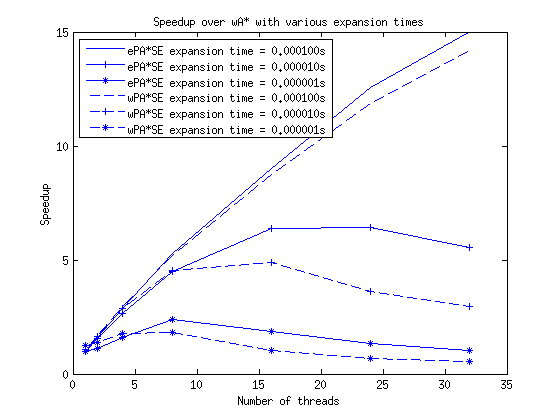
\includegraphics[scale=0.55]{time_sweep_all.png}
\caption{2D grid speedup as the number of threads and expansion time are varied.}
\end{figure}

\begin{figure}[fig:tps]
\centering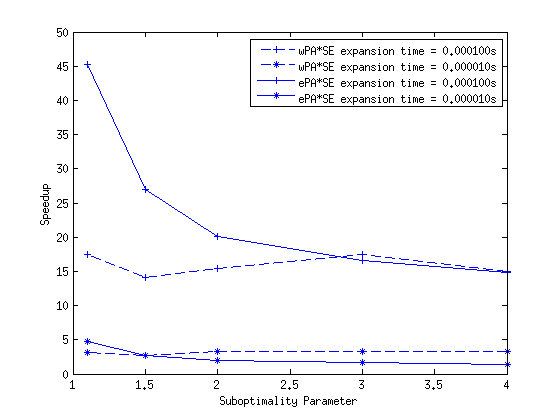
\includegraphics[scale=0.55]{eps_sweep_para.png}
\caption{2D grid speedup as the weight parameter and expansion time are varied.}
\end{figure}

\section{Conclusion}

We have presented a framework which unifies wA* and wPA*SE, differentiating them primarily by expansion rule. Within this framework, we created ePA*SE and proved it maintains the completeness and guaranteed bounded suboptimality of wPA*SE, with additional performance bounds in the limit of massive parallelism. We showed experimental gains in performance, presented an anytime variant, and discussed the role of decoupling the weight parameter from the suboptimality factor.

Future work remains to experimentally investigate the effect of using $w \ne \epsilon$ under various settings. The bottleneck of ePA*SE appears to be the fact that only one thread at a time can access the data structures to extract states. While prior work includes techniques for splitting the frontier for parallel access, none so far have all the theoretical benefits we showed for ePA*SE.

\bibliographystyle{aaai}
\bibliography{PAPA}

\end{document}
